\chapter{文件系统}

\section{文件操作}

\subsection{打开文件}

计算机除了拥有计算的能力之外,一定要有数据的存储能力,而对于数据的存储一般就可以通过文件的形式来完成。在Python中直接提供有文件的I/O(Input/Output)处理函数操作,利用这些函数可以方便地实现读取和写入。 \\

open()函数的功能是进行文件的打开,在进行文件打开的时候如果不设置任何的模式类型,则默认为r(只读模式)。

\begin{lstlisting}[language=Python]
def open(
    file, mode='r', buffering=None, encoding=None,
    errors=None, newline=None, closefd=True
)
\end{lstlisting}

\begin{table}[H]
	\centering
	\setlength{\tabcolsep}{5mm}{
		\begin{tabular}{|c|l|}
			\hline
			\textbf{模式} & \textbf{描述}                                  \\
			\hline
			r             & 使用只读模式打开文件,此为默认模式             \\
			\hline
			w             & 写模式,如果文件存在则覆盖,文件不存在则创建   \\
			\hline
			x             & 写模式,新建一个文件,如果该文件已存在则会报错 \\
			\hline
			a             & 内容追加模式                                   \\
			\hline
			b             & 二进制模式                                     \\
			\hline
			t             & 文本模式(默认)                               \\
			\hline
			+             & 打开一个文件进行更新(可读可写)               \\
			\hline
		\end{tabular}
	}
	\caption{文件打开模式}
\end{table}

如果以只读的模式打开文件,并且文件路径不存在的话,就会出现FileNotFoundError错误信息。 \\

\mybox{文件操作}
\begin{lstlisting}[language=Python]
def main():
    file = open(file="data.txt", mode="w")
    print("文件名称:%s" % file.name)
    print("访问模式:%s" % file.mode)
    print("文件状态:%s" % file.closed)
    print("关闭文件...")
    file.close()
    print("文件状态:%s" % file.closed)

if __name__ == "__main__":
    main()
\end{lstlisting}

\begin{tcolorbox}
	\mybox{运行结果} \\
	文件名称:data.txt \\
	访问模式:w \\
	文件状态:False \\
	关闭文件... \\
	文件状态:True
\end{tcolorbox}

\subsection{文件读写}

当使用open()打开一个文件之后,接下来可以使用创建的文件对象进行读写操作。 \\

使用读模式打开文件后,可以使用循环读取每一行的数据内容。Python在进行文件读取操作的时候也可以进一步简化操作。文件对象本身是可以迭代的,在迭代的时候是以换行符进行分割,每次迭代就读取到一行数据内容。

\begin{table}[H]
	\centering
	\setlength{\tabcolsep}{5mm}{
		\begin{tabular}{|l|l|}
			\hline
			\textbf{方法}                             & \textbf{描述}          \\
			\hline
			def close(self)                           & 关闭文件资源           \\
			\hline
			def fileno(self)                          & 获取文件描述符         \\
			\hline
			def flush(self)                           & 强制刷新缓冲区         \\
			\hline
			def read(self, n: int = -1)               & 数据读取,默认读取全部 \\
			\hline
			def readlines(self, hint: int = -1)       & 读取所有数据行         \\
			\hline
			def readline(self, limit: int = -1)       & 读取每行数据           \\
			\hline
			def truncate(self, size: int = None)      & 文件截取               \\
			\hline
			def writable(self)                        & 判断文件是否可以写入   \\
			\hline
			def write(self, s: AnyStr)                & 文件写入               \\
			\hline
			def writelines(self, lines, List[AnyStr]) & 写入一组数据           \\
			\hline
		\end{tabular}
	}
	\caption{文件读写方法}
\end{table}

既然所有的文件对象最终都需要被开发者关闭,那么可以结合with语句实现自动的关闭处理。通过with实现所有资源对象的连接和释放是在Python中编写资源操作的重要技术手段,通过这样的操作可以极大地减少和优化代码结构。 \\

\mybox{读取文件}
\begin{lstlisting}[language=Python]
def main():
    with open(file="data.txt", mode="r", encoding="utf-8") as file:
        for line in file:
            print(line, end='')

if __name__ == "__main__":
    main()
\end{lstlisting}

\begin{lstlisting}[language=Python, title=data.txt]
小灰	16
小白	17
小黄	21
\end{lstlisting}

\begin{tcolorbox}
	\mybox{运行结果} \\
	小灰	16 \\
	小白	17 \\
	小黄	21
\end{tcolorbox}

\vspace{0.5cm}
\mybox{写入文件}
\begin{lstlisting}[language=Python]
def main():
    with open(file="data.txt", mode="w", encoding="utf-8") as file:
        info = {"小灰": 16, "小白": 17, "小黄": 21}
        for name, age in info.items():
            file.write("%s\t%d\n" % (name, age))

if __name__ == "__main__":
    main()
\end{lstlisting}

\begin{tcolorbox}
	\mybox{运行结果} \\
	\textbf{data.txt} \\
	小灰	16 \\
	小白	17 \\
	小黄	21
\end{tcolorbox}

\newpage

\section{文件缓冲}

\subsection{文件缓冲}

在使用open()创建一个文件对象的时候,默认情况下是不会启用缓冲的。在open()中提供的buffering参数描述的就是文件处理缓冲的定义,在进行文件写入的时候利用缓冲可以避免频繁的I/O资源占用。 \\

开启缓冲可以提高写入效率,buffering参数设置有3种类型:

\begin{enumerate}
	\item 全缓冲(buffering > 1):当标准I/O缓存被填满后才会进行真正I/O操作,全缓冲的典型代表就是对磁盘文件的读写操作。

	\item 行缓冲(buffering = 1):在I/O操作中遇见换行符时才执行真正的I/O操作,例如在使用网络聊天工具时所编辑的文字在没有发送前是不会进行I/O操作的。

	\item 不缓冲(buffering = 0):直接进行终端设备的I/O操作,数据不经过缓冲保存。
\end{enumerate}

如果想要观察到行缓冲的使用特点,就不能直接使用with语句,因为with最后会执行close()的关闭操作,而一旦关闭,则缓冲的内容会全部进行输出。 \\

使用flush()进行缓冲区的强制清空,一旦强制清空之后,缓冲区的内容将全部输出。每次使用close()关闭文件流的时候默认情况下也会调用flush()进行缓冲区的清空处理。 \\

\mybox{文件缓冲}
\begin{lstlisting}[language=Python]
import os

def main():
    file = open(file="data.txt", mode="w",
                encoding="utf-8", buffering=1)
    file.write("This is a test.")
    os.system("pause")  # 程序暂停
    file.flush()        # 强制清空缓冲区
    os.system("pause")  # 程序暂停
    file.close()

if __name__ == "__main__":
    main()
\end{lstlisting}

\begin{tcolorbox}
	\mybox{运行结果} \\
	\textbf{data.txt} \\
	This is a test.
\end{tcolorbox}

\newpage

\section{文件系统}

\subsection{文件系统}

文件系统是OS中负责管理持久数据的子系统,也就是负责把用户的文件存到磁盘硬件中,即使计算机断电了,磁盘里的数据并不会丢失,所以可以持久化地保存文件。文件系统的基本数据单位是文件,它的目的是对磁盘上的文件进行组织管理。 \\

Linux最经典的一句话是``一切皆文件”,不仅普通的文件和目录,就连块设备、管道、socket等,也都是统一交给文件系统管理的。 \\

文件和目录是按照层次关系管理的,这种结构可以用树表示。文件夹中包含了子文件夹或者文件,这样就形成了一个树的结构。不过也有一些特殊情况,例如团队在协同工作时会共享一些信息,两个人有着不同的目录,但是可以共享同一份文件。 \\

Linux文件系统会为每个文件分配索引结点(inode)和目录项(directory entry)这两个数据结构。索引结点用来记录文件的元信息,比如inode编号、文件大小、访问权限、创建时间、修改时间、数据在磁盘的位置等。目录项用来记录文件的名字、索引结点指针以及与其它目录项的层级关联关系。多个目录项关联起来,就会形成目录结构,但它与索引结点不同的是,目录项是由内核维护的一个数据结构,不存放于磁盘,而是缓存在内存。 \\

由于索引结点唯一标识一个文件,而目录项记录着文件名,所以目录项和索引结点的关系是多对一。也就是说,一个文件可以有多个别名,例如,硬链接的实现就是多个目录项中的索引结点指向同一个文件。

\begin{figure}[H]
	\centering
	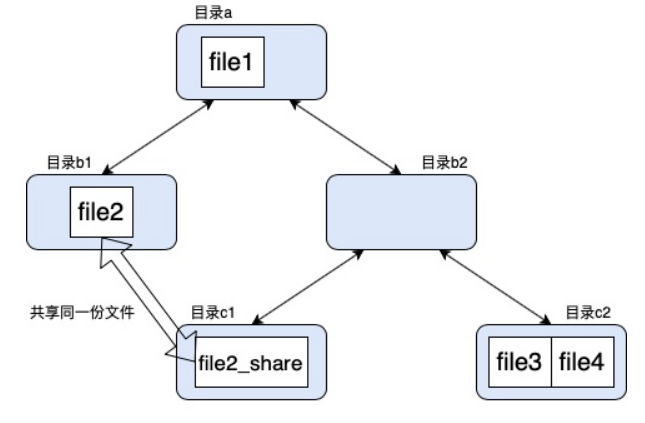
\includegraphics[scale=0.35]{img/C5/5-3/1.png}
	\caption{文件系统}
\end{figure}

\subsection{硬链接与软链接}

链接简单说实际上是一种文件共享的方式,主流文件系统都支持链接文件。链接简单地理解为Windows中常见的快捷方式,Linux中常用它来解决一些库版本的问题,通常也会将一些目录层次较深的文件链接到一个更易访问的目录中。 \\

链接分为硬链接(hard link)和软链接(symbolic link)。从使用的角度讲,两者没有任何区别,都与正常的文件访问方式一样,支持读写,如果是可执行文件的话也可以直接执行。 \\

硬链接通过同一个inode指向原始文件,软链接通过硬盘媒介中的描述指向原始文件。但是,当原始文件的位置发生改变后,inode不会改变,所以硬链接还是正确的,而软链接就无法访问了。

\begin{figure}[H]
	\centering
	\begin{tikzpicture}[scale=0.7]
		\draw[rounded corners] (0,0) rectangle (4,2);
		\draw[rounded corners] (6,0) rectangle (10,2);
		\draw[rounded corners] (12,0) rectangle (16,2);

		\draw (2,1) node {原始文件file1};
		\draw (8,1) node {硬链接file2};
		\draw (14,1) node {软连接file3};

		\draw[rounded corners] (2,-5) circle (2);
		\draw[rounded corners] (14,-5) circle (2);

		\draw (2,-4.5) node {inode};
		\draw (14,-4.5) node {inode};
		\draw (2,-5.5) node {37259183};
		\draw (14,-5.5) node {13549669};

		\draw[->] (2,0) -- (2,-3);
		\draw[->] (8,0) -- (2,-3);
		\draw[->] (14,0) -- (14,-3);
	\end{tikzpicture}
	\caption{硬链接与软链接}
\end{figure}

\newpage

\section{文件存储}

\subsection{顺序分配}

文件的数据是要存储在硬盘上面的,数据在磁盘上的存放方式,就像程序在内存中存放的方式那样,分为连续空间存放和非连续空间存放两种方式。不同的存储方式有各自的特点,它们的存储效率和读写性能各不相同。 \\

连续空间存放方式顾名思义,文件存放在磁盘连续的物理空间中。这种模式下,文件的数据都是紧密相连,读写效率很高,因为一次磁盘寻道就可以读出整个文件。 \\

使用连续存放的方式有一个前提,必须先知道一个文件的大小,这样文件系统才会根据文件的大小在磁盘上找到一块连续的空间分配给文件。所以文件头里需要指定起始块的位置和长度,有了这两个信息就可以很好地表示文件存放方式是一块连续的磁盘空间。

\begin{figure}[H]
	\centering
	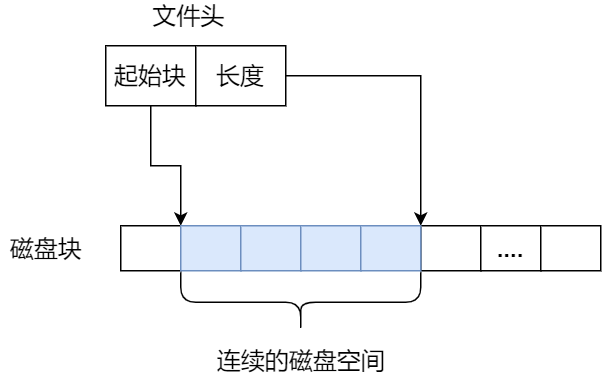
\includegraphics[scale=0.5]{img/C5/5-4/1.png}
	\caption{连续空间存放}
\end{figure}

连续空间存放的方式虽然读写效率高,但是有磁盘空间碎片和文件长度不易扩展的缺陷。

\begin{figure}[H]
	\centering
	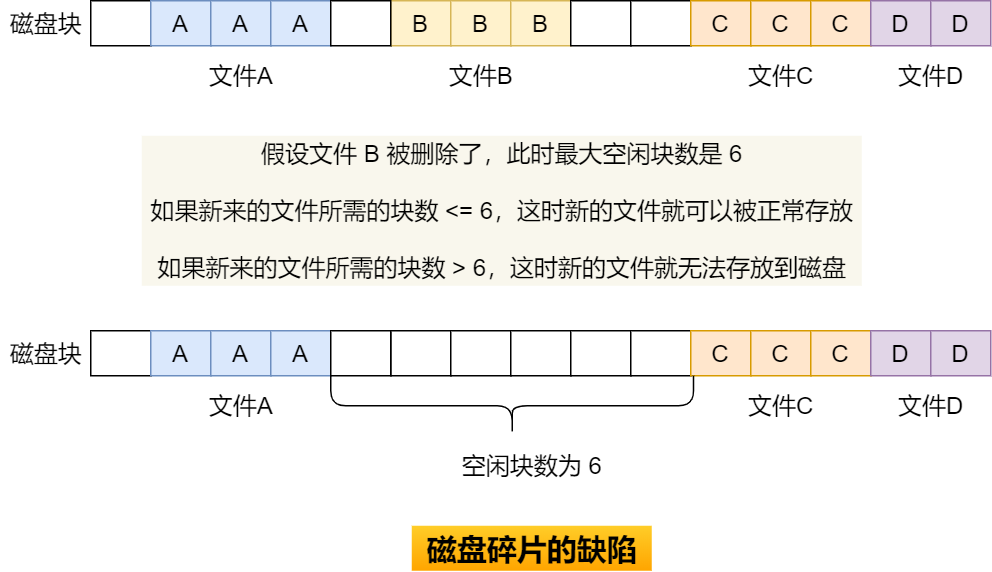
\includegraphics[scale=0.4]{img/C5/5-4/2.png}
	\caption{磁盘碎片}
\end{figure}

\subsection{链表分配}

链表的方式存放是离散的,于是就可以消除磁盘碎片,可大大提高磁盘空间的利用率,同时文件的长度可以动态扩展。根据实现的方式的不同,链表可分为隐式链表和显式链接两种形式。 \\

隐式链表实现的方式是文件头要包含第一块和最后一块的位置,并且每个数据块里面留出一个指针空间,用来存放下一个数据块的位置,这样从链头开始就可以顺着指针找到所有的数据块,所以存放是不连续的。

\begin{figure}[H]
	\centering
	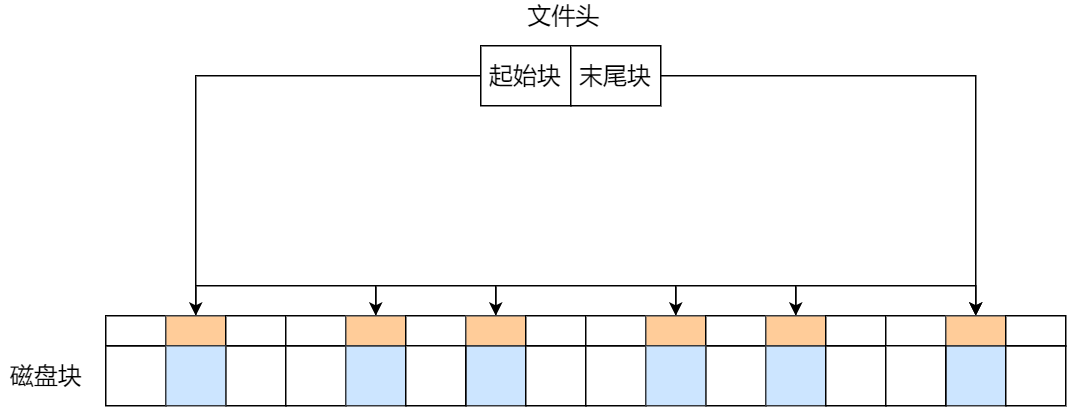
\includegraphics[scale=0.35]{img/C5/5-4/3.png}
	\caption{隐式链表存放}
\end{figure}

隐式链表存放方式的缺点在于无法直接访问数据块,只能通过指针顺序访问,以及数据块指针消耗了一定的存储空间。隐式链表稳定性较差,系统在运行过程中由于软件或者硬件错误导致指针丢失或损坏,会导致文件数据的丢失。 \\

如果取出每个磁盘块的指针,把它放在内存的一个表中,就可以解决上述隐式链表的两个不足。显式链接指把用于链接文件各数据块的指针,显式地存放在内存的一张链接表中,该表在整个磁盘仅设置一张,每个表项中存放链接指针,指向下一个数据块号。这个表格称为文件分配表(FAT, File Allocation Table)。

\begin{figure}[H]
	\centering
	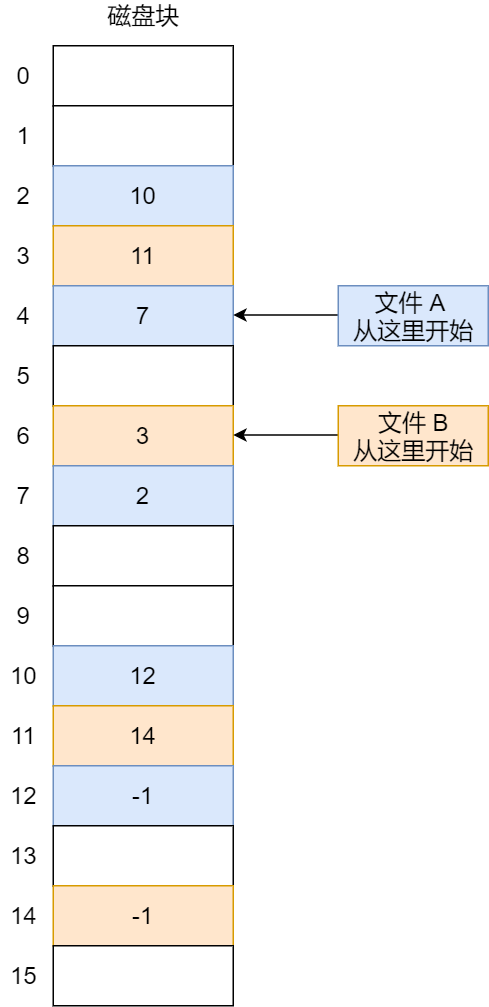
\includegraphics[scale=0.4]{img/C5/5-4/4.png}
	\caption{文件分配表FAT}
\end{figure}

\subsection{索引分配}

链表的方式解决了连续分配的磁盘碎片和文件动态扩展的问题,但是不能有效支持直接访问,索引的方式可以解决这个问题。索引的实现是为每个文件创建一个索引数据块,里面存放的是指向文件数据块的指针列表,类似于书的目录,通过目录就可以找到对应章节。文件头需要包含指向索引数据块的指针,这样就可以通过文件头知道索引数据块的位置,再通过索引数据块里的索引信息找到对应的数据块。

\begin{figure}[H]
	\centering
	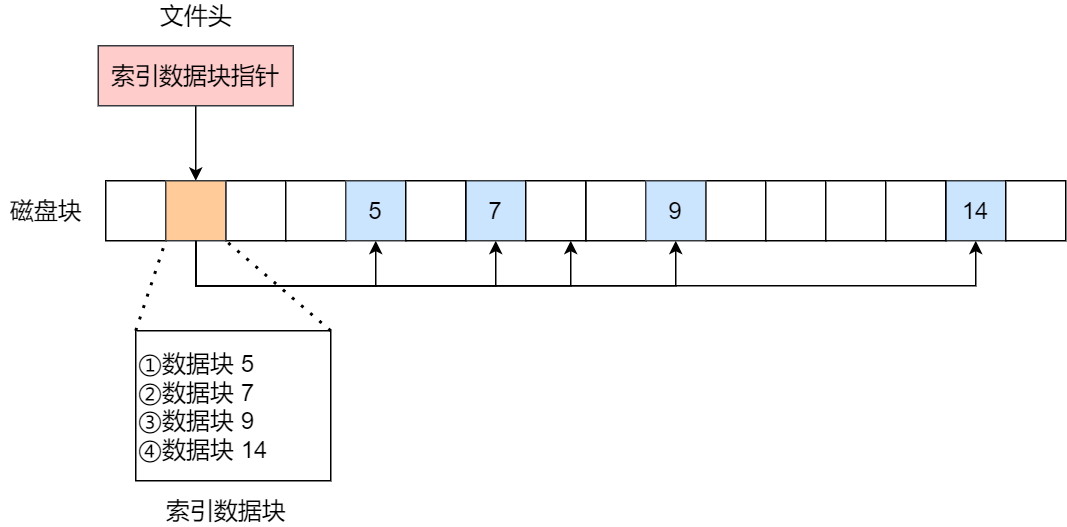
\includegraphics[scale=0.35]{img/C5/5-4/5.png}
	\caption{索引分配}
\end{figure}

索引的方式优点在于:

\begin{enumerate}
	\item 文件的创建、增大、缩小很方便
	\item 不会有碎片的问题
	\item 支持顺序读写和随机读写
\end{enumerate}

如果文件很大,大到一个索引数据块放不下索引信息,这时可以通过链表与索引的组合,这种组合称为链式索引块,它的实现方式是在索引数据块留出一个存放下一个索引数据块的指针,于是当一个索引数据块的索引信息用完了,就可以通过指针的方式,找到下一个索引数据块的信息。

\begin{figure}[H]
	\centering
	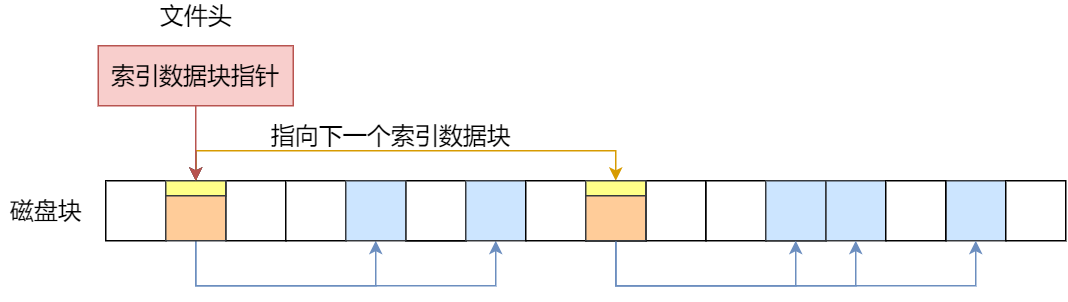
\includegraphics[scale=0.4]{img/C5/5-4/6.png}
	\caption{链式索引块}
\end{figure}

\newpage

\section{空闲空间管理}

\subsection{空闲表法}

文件的存储是针对已经被占用的数据块的组织和管理,如果要保存一个数据块,应该放在硬盘上的哪个位置呢?如果将所有的块扫描一遍寻找一个空闲空间,这种方式效率太低了,所以针对磁盘的空闲空间也要引入管理的机制。 \\

空闲表法就是为所有空闲空间建立一张表,表内容包括空闲区的第一个块号和该空闲区的块个数。注意,这个方式是连续分配的。

\begin{figure}[H]
	\centering
	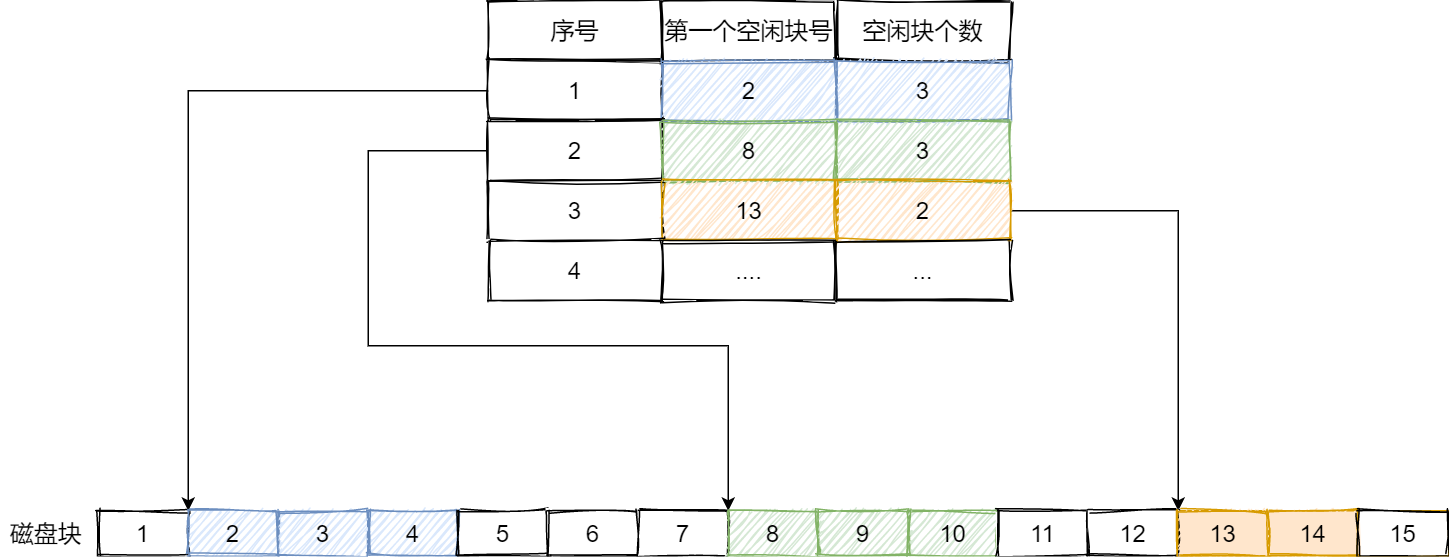
\includegraphics[scale=0.25]{img/C5/5-5/1.png}
	\caption{空闲表法}
\end{figure}

当请求分配磁盘空间时,系统依次扫描空闲表里的内容,直到找到一个合适的空闲区域为止。当用户撤销一个文件时,系统回收文件空间。这时,也需顺序扫描空闲表,寻找一个空闲表条目并将释放空间的第一个物理块号及它占用的块数填到这个条目中。 \\

这种方法仅当有少量的空闲区时才有较好的效果,因为如果存储空间中有着大量的小的空闲区,则空闲表变得很大,这样查询效率会很低。另外,这种分配技术适用于建立连续文件。

\subsection{空闲链表法}

除了空闲表,也可以使用链表的方式来管理空闲空间,每一个空闲块里有一个指针指向下一个空闲块,这样也能很方便的找到空闲块并管理起来。当创建文件需要一块或几块时,就从链头上依次取下一块或几块。反之,当回收空间时,把这些空闲块依次接到链头上。

\begin{figure}[H]
	\centering
	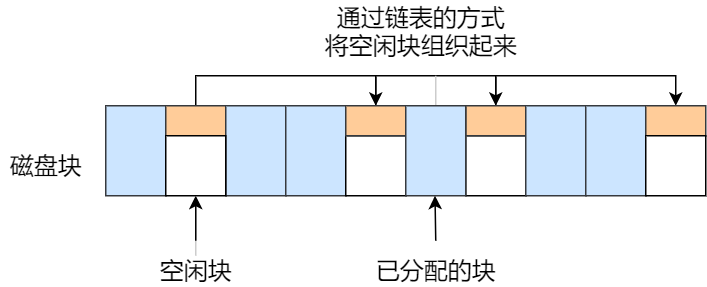
\includegraphics[scale=0.5]{img/C5/5-5/2.png}
	\caption{空闲链表法}
\end{figure}

这种技术只要在主存中保存一个指针,令它指向第一个空闲块。其特点是简单,但不能随机访问,工作效率低,因为每当在链上增加或移动空闲块时需要做很多I/O操作,同时数据块的指针消耗了一定的存储空间。 \\

空闲表法和空闲链表法都不适合用于大型文件系统,因为这会使空闲表或空闲链表太大。

\subsection{位图法(Bit Table)}

位图是利用二进制的一位来表示磁盘中一个盘块的使用情况,磁盘上所有的盘块都有一个二进制位与之对应。当值为0时,表示对应的盘块空闲,值为1时,表示对应的盘块已分配。Linux文件系统就采用了位图的方式来管理空闲空间。